\pagebreak
\section{Background for Architectural Design Dimension}
\label{sec:background-architectural-design}

Modern software architecture treats modularity as a primary mechanism for balancing immediate development needs with long-term scalability. In the context of a modular monolith, this means structuring the application as a single deployable unit that internally consists of well-defined, self-contained modules. Each module acts as a building block of the system, encapsulating a cohesive set of related functionality behind a clear boundary. By imposing strict internal module boundaries and interfaces, a modular software design approach can preserve many benefits commonly associated with more distributed architectures, such as parallel development by multiple engineering teams, maintainability, and scalability, while avoiding a substantial portion of the operational complexity of distributed systems \cite{abgaz2023decomposition, grzybek2020modular}. The monolith's internals are made scalable and maintainable by design, and the system remains ready for gradual growth or future distribution, enabling progressive scalability \cite{grzybek2020modular}. Recent systematic reviews confirm growing academic interest in this architectural style, with Al-Qora'n and Al-Said Ahmad~\cite{alqoran2025mma} surveying modular monolith adoption in cloud environments, and Su and Li~\cite{su2024modular} examining whether the modular monolith represents an emerging trend in software architecture. In summary, modular monolith architecture aims to achieve scalability and maintainability through disciplined modular boundaries within a single deployable unit.

\begin{figure}[H]
  \centering
  \includegraphics[width=0.90\linewidth]{Cap4/guidelines/modular-deployment-units.png}
  \caption[Deployment units in modular monoliths and microservices]{Deployment units in modular monoliths and microservices. The left side illustrates a modular monolith, where domain-aligned modules (e.g., Orders, Users, Payments, Inventory) execute within a single runtime and may share a single data store, while enforcing internal boundaries through code-level constraints. The right side illustrates microservices, where each service runs as an independent runtime and typically owns its persistence, enabling independent deployment and scaling at the cost of distributed-system operational overhead. Source: Dr Milan Milanović (adapted for this research).}
  \label{fig:modular-deployment-units}
\end{figure}

\pagebreak
Against this background, the discussion that follows places emphasis on the Architectural Design dimension. This research proposes that progressive scalability in modular monoliths depends first on enforceable modularity, meaning clear boundaries, explicit contracts, and build or test-time checks that detect boundary corruption early.

This priority also shapes the guideline order. The guidelines are presented by impact, with G1 as the foundation: without verifiable boundary enforcement, later guidelines are harder to apply because they assume stable module interfaces and controlled coupling. For that reason, this section introduces the concepts needed for the Architectural Design guidelines, including modular decomposition styles, coupling and cohesion, screaming architecture, layering, packaging strategies, and module design principles. The goal is to make explicit how coupling patterns affect the cost of change, and why domain-centric modularity helps sustain cohesion over time.

A useful way to frame architectural design is as an evolutionary progression in separation of concerns. Early architectural organization frequently optimized for technical separation, for example MVC and layered structures. Over time, the emphasis shifted toward dependency discipline and domain centric organization, as seen in Hexagonal Architecture, Onion Architecture, and Clean Architecture \cite{cockburn2005hexagonal,palermo2008onion,martin2012clean}.

\begin{figure}[H]
  \centering
  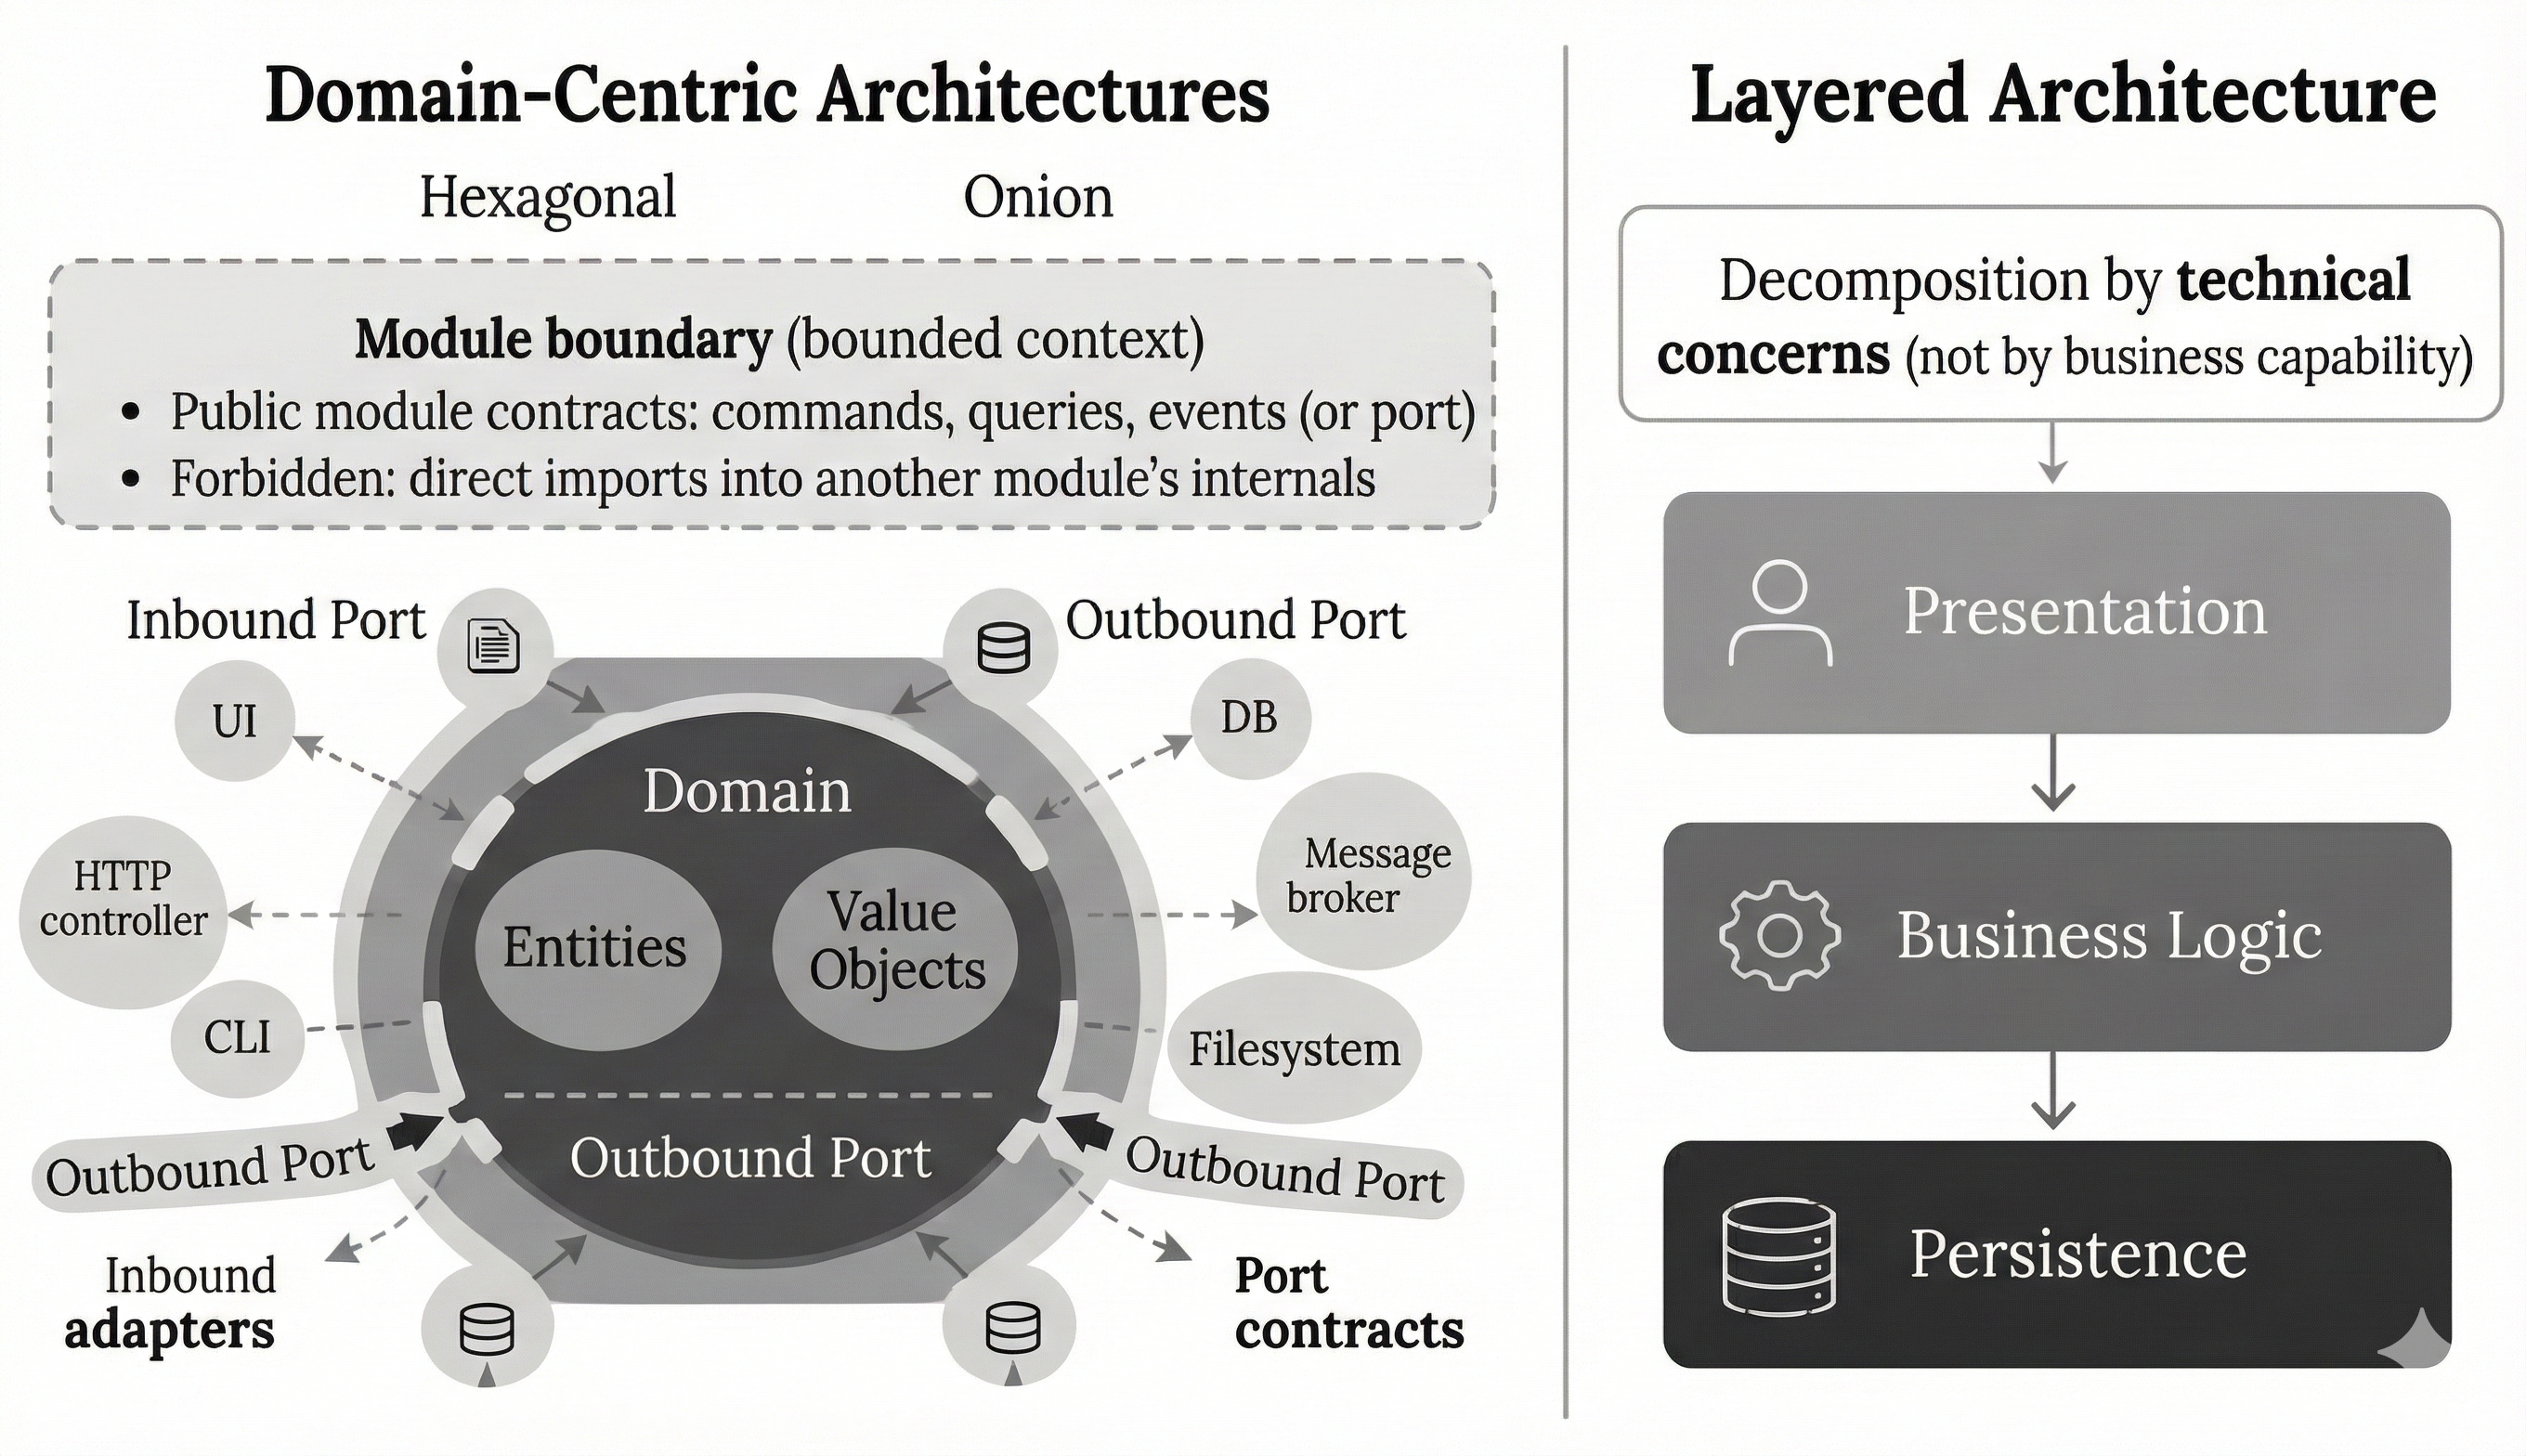
\includegraphics[width=0.75\linewidth]{Cap4/guidelines/domain-centric-layered-arch.png}
  \caption[Layered architecture versus domain-centric architecture]{Layered versus domain-centric architecture. This representation supports the argument that domain-centric shifts the primary decomposition axis from technical layers to business capabilities, with the goal of improving cohesion and reducing cross-cutting coupling.}
  \label{fig:layered-vs-domain-architecture}
\end{figure}

In parallel, packaging strategies evolved from technical layers to feature slices, and then to component-like modules that align more directly with domain boundaries \cite{shaw2018vertical}. Comparative studies such as Hmue et al.~\cite{hmue2024microservices} reinforce this trajectory by showing that monolithic and microservice architectures involve distinct trade-offs in web development, motivating intermediate approaches that preserve monolithic simplicity while introducing modular discipline. This research proposal positions modular monolith guidelines as a pragmatic state of practice that combines these influences, aiming to control change cost by constraining coupling and making boundaries verifiable in code.

% [FIGURE:evolution-of-architectures]
% Placeholder for an evolutionary timeline diagram (e.g., MVC, layered, Hexagonal, Onion, Clean Architecture,


\subsection*{Cost of Change: Coupling and Cohesion}

Cost of change is often dominated by dependency structure rather than by local code complexity. As Russell L. Ackoff argues, \textit{"A system is never the sum of its parts, it's the product of their interactions."} This perspective motivates treating coupling patterns as first order architectural concerns, because interactions are where change propagates, coordination increases, and unintended side effects emerge.

When introducing coupling and cohesion, this research proposal explicitly draws on the structured design foundations of Edward Yourdon and Larry Constantine, whose work provides a rigorous vocabulary for understanding how dependency structure shapes maintainability and change amplification \cite{yourdon1979structured}. Their framing is used here to examine three claims that are central to the Architectural Design Dimension (G1--G3):

\begin{itemize}
    \item \textbf{Not all coupling is born equal.} Some dependencies are stabilizing and intentional, particularly inside a coherent boundary, while others are accidental and create ripple effects across unrelated areas.
    \item \textbf{Decoupling has its cost.} Indirection, abstractions, and additional interfaces can reduce harmful dependency, but may increase cognitive load and implementation overhead if applied without need.
    \item \textbf{Cohesion is coupling in the right places.} Coupling is not eliminated, it is relocated into cohesive units so that change remains localized.
\end{itemize}

These claims motivate a baseline definition of what \textit{"good modularity"} is aimed at in this research. Software design can be treated as the act of modeling units of \textbf{strong cohesion, loosely coupled} to each other. The Architectural Design Dimension (G1--G3) operationalizes this by proposing guidelines that make coupling explicit, constrain it through boundary rules, and preserve cohesion by aligning modules with business capabilities rather than technical utilities.

This framing also clarifies why domain centric modularity is emphasized. Functional decomposition is generally preferred over technical decomposition when the goal is to reduce change amplification, because it tends to localize business evolution inside a bounded unit. This directly relates to the distinction between intrinsic complexity, which comes from the domain and requirements, and accidental complexity, which comes from architectural and organizational choices. A recurring risk in modularization is mistaking organization for encapsulation, because directory structure alone does not enforce boundaries unless it is backed by interface contracts and dependency rules.

\subsection*{Modular Decomposition Styles: Horizontal vs Vertical}
A fundamental design decision concerns how system functionality is decomposed. The two primary strategies are horizontal decomposition, organized by technical layer, and vertical decomposition, organized by feature or business capability. In traditional layered architectures, code is structured by technical responsibilities such as presentation, application services, and persistence. While this approach provides a form of separation of concerns, it often disperses domain logic across multiple layers and obscures the system's business intent \cite{fowler2002}. Fowler~\cite{fowler2015presentationdomaindatalayering} further argues that the presentation--domain--data layering pattern, though useful as a starting heuristic, tends to scatter domain logic when applied rigidly across a growing codebase. As a result, understanding or modifying a specific feature frequently requires coordinated changes across several layers.

This change amplification effect can be stated directly. Changes to a layered architecture usually result in changes across all layers. The reason is that the dependency structure encourages features to cut across horizontal boundaries, even when the business change is conceptually localized. This coupling pattern increases the long term cost of change, because each new behavior requires cross layer coordination, additional integration effort, and broader regression risk.

\begin{figure}[H]
  \centering
  \includegraphics[width=0.45\linewidth]{Cap4/guidelines/change-coupled-effect.png}
  \caption[Coupled-change ripple in a dependency graph]{Coupled-change ripple in a dependency graph. Nodes represent components and directed edges represent dependencies. The change originates at the top node (annotated as the starting point) and propagates along dependency paths. Darker nodes indicate components impacted by the initial modification, while lighter nodes remain unaffected. Concentric halos emphasize the spread of change through the system, illustrating how tighter coupling amplifies change impact beyond the original change.}
  \label{fig:change-coupling-ripple}
\end{figure}


Vertical decomposition addresses this limitation by organizing code around features, use cases, or domain capabilities. All elements required to implement a specific behavior, including API endpoints, business logic, and data access, are grouped within a single module or slice. This approach is commonly referred to as package by feature or vertical slice architecture \cite{shaw2018vertical}. By aligning structural boundaries with business concepts, vertical decomposition tends to increase cohesion, reduce cross feature coupling, and make related code easier to find, because feature behavior is not scattered across horizontal layers.

\begin{figure}[H]
  \centering
  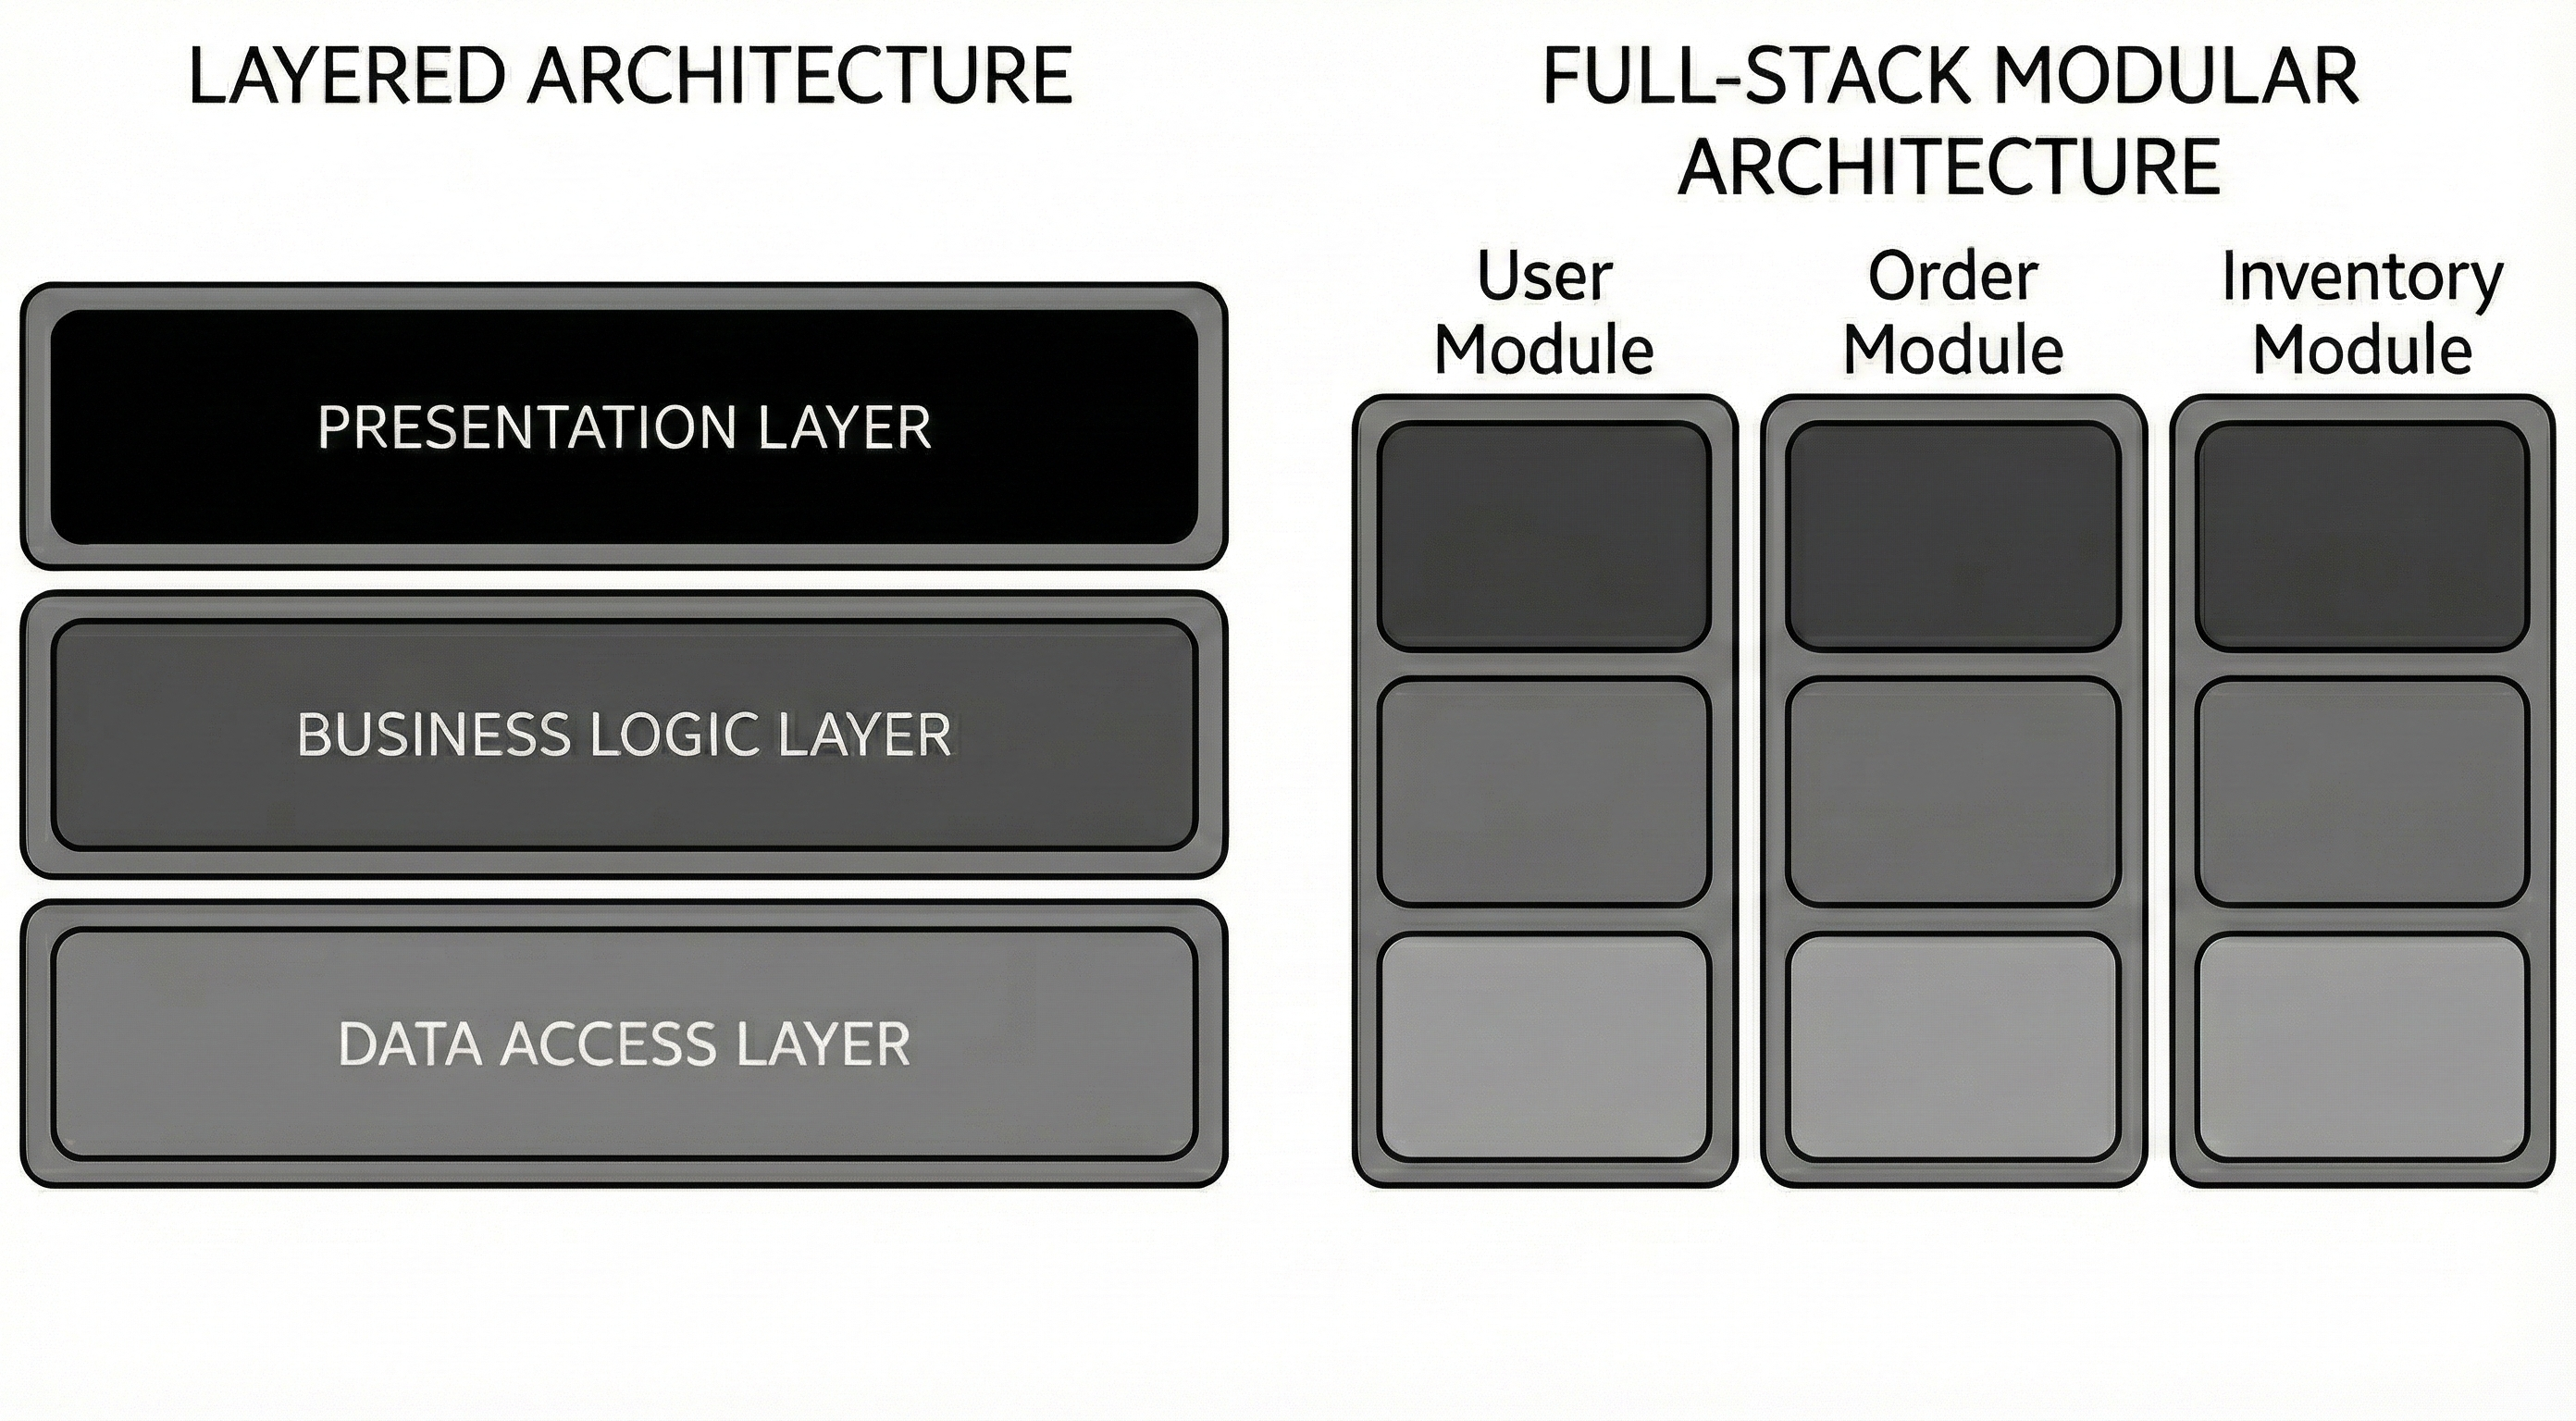
\includegraphics[width=0.8\linewidth]{Cap4/guidelines/layered-vs-modular.png}
  \caption[Layered and modular architecture]{Layered and modular architecture. The left side shows a traditional layered decomposition, where code is organized by technical responsibility (presentation, business logic, and data access). The right side shows a modular decomposition, where domain modules (for example, User, Order, and Inventory) each contain their own UI/API, application logic, and persistence concerns, keeping feature changes more localized within module boundaries.}
  \label{fig:layered-vs-modular}
\end{figure}


A key risk at this stage is architectural \textit{"cargo culting"}, where teams adopt a packaging style or pattern without understanding the coupling problem it is intended to solve. It can also refer to the results of applying a design pattern or coding style blindly without understanding the reasons behind that design principle. In practice, this risk is elevated when architecture is documented as diagrams but not enforced in code, because teams can claim domain boundaries while the implementation continues to couple through shared models, utilities, or unrestricted imports.

\pagebreak

\subsection*{Screaming Architecture: Domain Alignment and Model--Code Gap}

A \emph{screaming architecture} is one in which the system's structure communicates its business purpose at a glance. A well-designed codebase foregrounds domain concepts and use cases in its top-level organization, rather than privileging frameworks, infrastructure, or technical layering \cite{martin2012clean,martin2011screaming}. Under this view, architecture is expressed less by diagrams and more by what the source code organization makes immediately visible, what the codebase ``\textit{screams}'' becomes a proxy for architectural intent.

This perspective is particularly relevant to the Architectural Design Dimension (G1--G3), where modular boundaries are treated as first-class architectural elements. When the dominant structural signals emphasize technical concerns instead of domain concepts, the system tends to drift away from domain-centric modularity. Over time, this drift increases the cost of change, since engineers must reconstruct domain intent from dispersed artifacts, raising cognitive load and coordination overhead.

This risk connects to the \emph{model--code gap} \cite{fairbanks2010justenough}, the divergence between an architecture as documented and an architecture as implemented. Fairbanks argues that when architectural decisions are not made evident in code, they erode under delivery pressure, producing systems that appear compliant in documentation while contradicting the intended structure in practice.

To reduce this gap, Fairbanks proposes an \emph{architecturally-evident coding style}, where architectural decisions are encoded directly into module boundaries and enforced dependency rules \cite{fairbanks2010justenough}. Mechanisms include explicit public interfaces, restricted import paths, and structural checks that fail when dependency constraints are violated. A central implication for this research is that modular boundaries should be explicit, inspectable, and continuously enforced by the codebase, making violations difficult to introduce unintentionally.

\begin{figure}[H]
  \centering
  \includegraphics[width=0.70\linewidth]{Cap4/guidelines/explicit-modular-boundary.png}
  \caption[Explicit modular boundary with enforced imports]{Explicit modular boundary with enforced imports.}
  \label{fig:explicit-modular-boundary}
\end{figure}


\pagebreak
An example of what a screaming architecture looks like in practice is illustrated by the high-level directory structure that will be explored in detail in the guideline examples. Even without inspecting individual files or previous knowledge of the codebase, the system's domain and capabilities are immediately apparent:

\lstset{
  basicstyle=\ttfamily\small,
  columns=fullflexible,
  keepspaces=true,
  showstringspaces=false,
  frame=single,
  framerule=0.3pt,
  xleftmargin=0.5cm,
  xrightmargin=0.5cm
}

\begin{lstlisting}
|-- /modules/                  # Bounded contexts represented in Modules
|   |-- orders/
|   |   |-- domain/
|   |   |   |-- entities/          # Order aggregate
|   |   |   |-- value-objects/     # OrderItem, CustomerId
|   |   |   |-- events/            # Domain events
|   |   |   +-- repositories/      # OrderRepository (database operations)
|   |   |-- features/             # Use cases (vertical slices)
|   |   |   |-- place-order/           # Place Order services/use-cases
|   |   |   +-- cancel-order/          # Cancel Order services/use-cases
|   |   +-- listeners/             # Event handlers of Orders
|   |-- inventory/                # Inventory module
|   |-- payments/                 # Payments module
|   +-- shipments/                # Shipments module
\end{lstlisting}

At this level, the architecture already ``\textit{screams}'' business capabilities such as orders, inventory, payments, and shipments, rather than technical layers or framework concerns. This structure makes domain boundaries, use cases, and integration points visible by construction, reducing the model--code gap before any implementation details are examined.

Within this research, screaming architecture and the model--code gap are treated as two facets of the same underlying problem. Architecture that exists only in documentation is fragile and prone to corruption. Architecture that is embedded in module boundaries, public APIs, and enforced dependency direction becomes continuously verifiable. This embedded nature is a prerequisite for controlling coupling, sustaining cohesion, and supporting progressive scalability within a modular monolith, and directly informs the Architectural Design Dimension (G1--G3) introduced in the following sections.

\pagebreak
\subsection*{Separation of Concerns and Dependency Discipline}

Separation of concerns can be implemented through architectural styles that constrain dependency direction. Layered Architecture typically structures dependencies outward to inward by technical responsibility, often represented as Presentation, Business, and Persistence layers \cite{fowler2002}. While layering can improve local reasoning, it may also amplify change cost when features cut across layers and when domain logic is fragmented into anemic models and service orchestration.

Hexagonal Architecture, Onion Architecture, and Clean Architecture formalize a stricter dependency rule: business logic is insulated from delivery and infrastructure concerns, and dependencies must point inward toward stable domain abstractions \cite{cockburn2005hexagonal,palermo2008onion,martin2012clean}. A common representation of this structure is:

\begin{figure}[H]
  \centering
  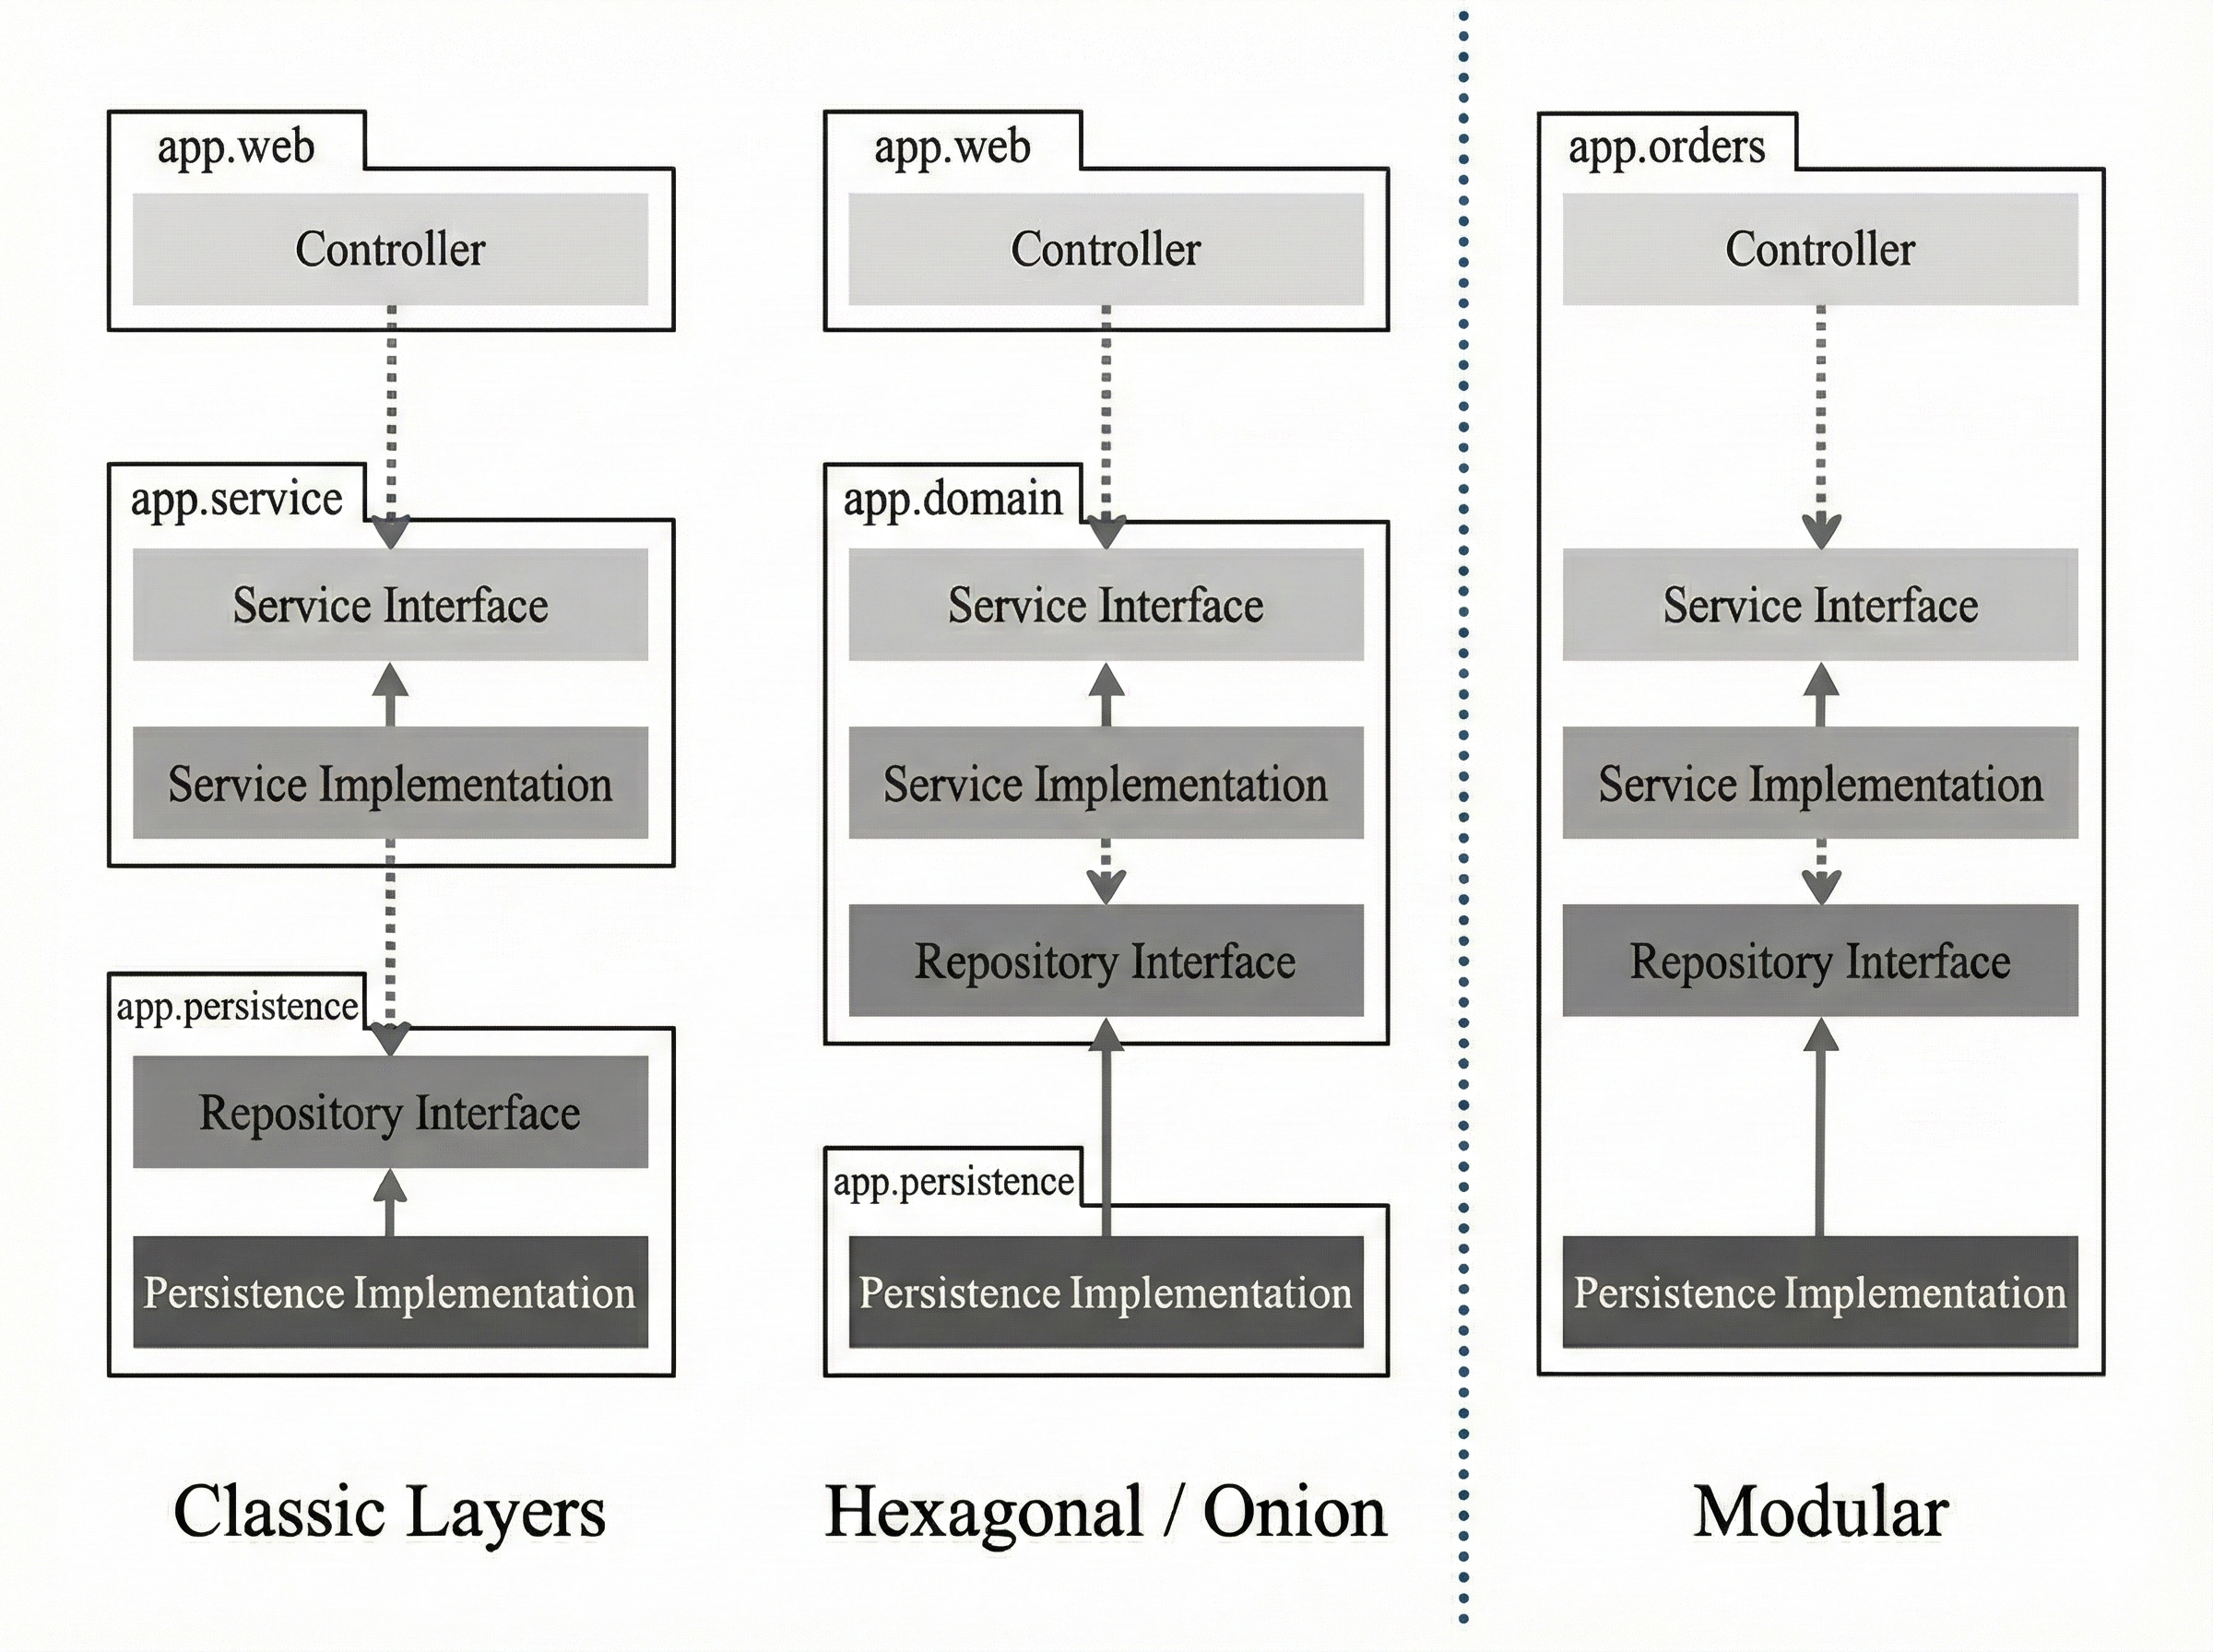
\includegraphics[width=0.95\linewidth]{Cap4/guidelines/hexa-onion-modular.png}
  \caption[From layered to modular architecture styles]{Comparison of architectural decomposition styles.}
  \label{fig:layered-vs-hexagonal-vs-modular}
\end{figure}


The intent is to reduce coupling to volatile infrastructure by inverting dependencies through interfaces and ports. This can reduce change cost because infrastructure replacements, testing strategies, and delivery mechanisms can evolve without rewriting core domain logic. However, dependency discipline alone does not guarantee domain centric modularity. A codebase can follow inward dependencies and still be organized as a single, tightly coupled domain blob if boundaries between business capabilities are not explicit.


\subsection*{Packaging and Slicing Strategy}
Packaging strategy determines what coupling is easy and what coupling is discouraged. This section compares three strategies using consistent terminology, because the Architectural Design Dimension (G1--G3) depends on understanding what each strategy optimizes for and where it tends to fail.

Package by layer is a horizontal slicing where code is organized by what it does from a technical perspective, such as controllers, services, repositories, and shared models. Traditional MVC architectures typically follow this approach, grouping responsibilities according to technical roles rather than business capabilities.

The primary failure mode is that business changes often span multiple technical packages, increasing coordination and regression risk. In layered architectures, even localized changes typically propagate across presentation, application, and persistence layers, amplifying the cost of change. This approach is closely associated with the model-code gap, since domain boundaries may be articulated in documentation while the code structure instead emphasizes technical layers.

This failure mode is reinforced by delivery-driven optimization, where short-term convenience encourages cross-layer shortcuts and shared abstractions. As business behavior evolves, conceptually narrow changes tend to trigger multi-layer modifications, increasing change amplification and obscuring architectural intent.

Because domain boundaries remain implicit and unenforced in the code, the system gradually reflects technical decomposition rather than business capability, widening the model-code gap and weakening the sustainability of modular reasoning.

\begin{figure}[H]
  \centering
  \includegraphics[width=0.80\linewidth]{Cap4/guidelines/package-by-layer-dir.png}
\end{figure}

Package by feature is a vertical slicing where code is organized by what it does from a functional perspective, including features, domain concepts, use cases, and aggregate roots. Cited benefits include higher cohesion, lower coupling, and related code being easier to find, because the implementation of a behavior is localized rather than scattered across technical packages \cite{shaw2018vertical}.

A common failure mode is turning features into an unstructured set of folders without stable interfaces, which can reintroduce hidden coupling through shared utilities and unrestricted imports. In such cases, vertical structure exists superficially, but architectural boundaries remain unenforced.

Another side-effect failure arises when nominal module boundaries are introduced without corresponding ownership of data and behavior. In these cases, modules expose internal state through shared data models, common persistence schemas, or cross-module service calls that bypass defined interfaces. Although the codebase may appear modular at the directory level, effective encapsulation is absent, allowing changes in one module to ripple unpredictably into others.

This pattern undermines substitutability and independent evolution, and it often emerges when modularization is treated as a structural refactoring exercise rather than as an architectural commitment enforced through explicit contracts and dependency constraints.

\begin{figure}[H]
  \centering
  \includegraphics[width=0.80\linewidth]{Cap4/guidelines/package-by-feature-dir.png}
\end{figure}

\pagebreak
Package by component is a packaging strategy in which code is organized around cohesive components, grouping functionality related to a specific responsibility. A component is defined as a unit of related behavior, accessed through a well-defined interface and encapsulated within the application boundary. This approach applies component-based or service-oriented design principles to a monolithic codebase, aiming to achieve modularity without introducing distribution.

The architectural hypothesis is that component boundaries become enforceable when they define what is exposed publicly, what is hidden internally, and which dependency directions are permitted between components. Under these conditions, package by component is the closest analogue to modules in a modular monolith architecture, where boundaries are enforceable constraints rather than organizational conventions, and coupling is intentionally limited.

A common failure mode arises when components are defined without a clear domain model, instead of being aligned with bounded contexts and aggregates as proposed in Domain-Driven Design \cite{evans2003ddd}. Overly coarse components collapse multiple domain concepts into a single unit, accumulating unrelated responsibilities and reintroducing hidden coupling through shared models. Conversely, overly fine-grained components fragment aggregates and use cases across boundaries, increasing coordination overhead and weakening invariants that should be preserved within a single consistency boundary. In both cases, the absence of stable, intention-revealing interfaces grounded in explicit domain contracts undermines boundary enforcement, allowing dependencies to leak through shared abstractions or convenience-driven imports. As a result, components may exist as structural groupings without providing the isolation, autonomy, and scalability expected of modular units in a modular monolith.

\begin{figure}[H]
  \centering
  \includegraphics[width=0.80\linewidth]{Cap4/guidelines/package-by-component.png}
\end{figure}

\subsection*{Modularity as an Enforceable Principle}

Modularity is treated in this research as an enforceable property rather than as a folder convention. Encapsulation and information hiding remain core mechanisms, because they minimize the number of potential dependencies by reducing what other modules can see and use \cite{parnas1972informationhiding}. This implies several practical principles that the Architectural Design Dimension (G1--G3) later operationalizes:

\begin{itemize}
    \item Separating interface from implementation. Modules should expose a small public API and keep internal details private.
    \item Using encapsulation to minimize dependencies. Fewer public types and fewer cross-module imports reduce change propagation paths.
    \item Matching public surface area to architectural intent. The surface area of internal public APIs and event listeners should reflect intended coupling and allowed integration points.
    \item Splitting the source code tree into multiple parts. Organizing the codebase into explicit module roots, for example /modules, helps architectural visibility and makes boundary enforcement feasible, because module ownership and dependency direction can be checked.
\end{itemize}

This view also reinforces the earlier distinction between organization and encapsulation. \textbf{Encapsulation over organization} means that directory structure matters only to the extent that it is backed by dependency rules, stable interfaces, and verification mechanisms. Without enforcement, modularity claims tend to collapse under delivery pressure, and coupling becomes implicit again.

Tiny Store's code repository \footnote{\url{https://github.com/maurcarvalho/tiny-store}} reflects the architectural hypothesis of modular boundaries and serves as a concrete artifact grounding the concepts introduced in this chapter. The project is publicly available and maintained as a reference implementation for this research, providing an auditable codebase in which packaging strategies and boundary enforcement mechanisms can be inspected directly.

The codebase is split into multiple parts that make architectural boundaries explicit, including a dedicated API layer and bounded context modules, with clearly defined locations for feature slices and for cross-module integration through domain events. Although this chapter does not yet rely on detailed implementation examples, the repository is introduced here to ensure that the vocabulary and architectural constructs discussed in the Architectural Design Dimension (G1--G3) are mapped to concrete verifiable structures instead of remaining purely conceptual.


\subsection*{Definition of Module Quality}

The Architectural Design Dimension (G1--G3) treats module quality as a measurable architectural objective. Modules are therefore expected to satisfy the following properties:

\begin{itemize}
    \item High cohesion and Low coupling
    \item Focused on a specific self contained business capability
    \item Aligned to a bounded context or aggregate
    \item Encapsulated data
    \item Substitutable
    \item Composable with other modules
\end{itemize}

This checklist is used later as the baseline for designing boundaries, for defining public APIs and events, and for evaluating whether a proposed module decomposition is likely to reduce change cost rather than merely reshuffle code.

\subsection*{Practical Evaluation for the Architectural Design Dimension (G1--G3)}

This foundations chapter establishes a causal chain that the guideline templates and their verification plans will later operationalize. Coupling patterns dominate change cost, cohesion localizes change, separation of concerns reduces dependency on volatile infrastructure, and packaging strategy determines whether the code structure screams domain intent or technical layers. Modularity becomes sustainable only when interfaces, dependency direction, and enforcement mechanisms make boundaries explicit and verifiable.

In the next sections, the Architectural Design Dimension (G1--G3) will translate these foundations into guideline templates that specify intent, rationale, applicability conditions, supported by Tiny Store codebase as a reference artifact for reproducibility of examples and auditability convenience.

% Note: fairbanks2010justenough is in referencias.bib